\documentclass[runningheads,a4paper,11pt]{report}

\usepackage{algorithmic}
\usepackage{algorithm} 
\usepackage{array}
\usepackage{amsmath}
\usepackage{amsfonts}
\usepackage{amssymb}
\usepackage{amsthm}
\usepackage{caption}
\usepackage{comment} 
\usepackage{epsfig} 
\usepackage{fancyhdr}
\usepackage[T1]{fontenc}
\usepackage{geometry} 
\usepackage{graphicx}
\usepackage[colorlinks]{hyperref} 
\usepackage[latin1]{inputenc}
\usepackage{multicol}
\usepackage{multirow} 
\usepackage{rotating}
\usepackage{setspace}
\usepackage{subfigure}
\usepackage{url}
\usepackage{verbatim}
\usepackage{xcolor}
\usepackage[export]{adjustbox}

\geometry{a4paper,top=3cm,left=2cm,right=2cm,bottom=3cm}

\pagestyle{fancy}
\fancyhf{}
\fancyhead[L,RO]{Automated Assistant for Medical Students and Doctors}
\fancyhead[R,LO]{Pinguinii Galactici}
\fancyfoot[R,LO]{ITSG 2020-2021}
\fancyfoot[L,RO]{\thepage}

\renewcommand{\headrulewidth}{2pt}
\renewcommand{\footrulewidth}{1pt}
\renewcommand{\headrule}{\hbox to\headwidth{%
  \color{lime}\leaders\hrule height \headrulewidth\hfill}}
\renewcommand{\footrule}{\hbox to\headwidth{%
  \color{lime}\leaders\hrule height \footrulewidth\hfill}}

\hypersetup{
pdftitle={artTitle},
pdfauthor={name},
pdfkeywords={pdf, latex, tex, ps2pdf, dvipdfm, pdflatex},
bookmarksnumbered,
pdfstartview={FitH},
urlcolor=cyan,
colorlinks=true,
linkcolor=red,
citecolor=green,
}

\setcounter{secnumdepth}{3}
\setcounter{tocdepth}{3}

\linespread{1}

\makeindex


\begin{document}

\begin{titlepage}
\sloppy

\begin{center}
BABE\c S BOLYAI UNIVERSITY, CLUJ NAPOCA, ROM\^ ANIA

FACULTY OF MATHEMATICS AND COMPUTER SCIENCE

\vspace{6cm}

\Huge \textbf{Automated Assistant for Medical Students and Doctors}

\vspace{1cm}

\normalsize -- ITSG report --

\end{center}


\vspace{5cm}

\begin{flushright}
\Large{\textbf{Team members}}\\
Mircea Maria-Madalina, Applied Computational Intelligence, 256

Moisuc Naomi, Software Engineering, 258

Jugaru Robert-George, Software Engineering, 258
\end{flushright}

\vspace{4cm}

\begin{center}
2020-2021
\end{center}

\end{titlepage}

\pagenumbering{gobble}

\begin{abstract}

Cancer is a life-threatening disease with a high mortality rate. Tumors can grow in any tissue and they can go unnoticed for a long time, perhaps until it is too late to save the patient's life. Early detection is paramount for the hope of a full recovery. 

This paper proposes a Mask-RCNN approach to the segmentation of tumors in MRI scans of the urinary bladder. The evaluation metrics we obtain prove that an automated approach is the way to go when it comes to early cancer diagnosis. 

This paper also applies the same principle to the segmentation of the prostate. The results suggest that there is a need for a more comprehensive, general, and high-quality dataset for this task.

The intelligent models are then integrated into a user-friendly web application that can assist doctors, doctors in training, and students identify bladder tumors in NRRD files and PNG images.
	
\end{abstract}


\tableofcontents

\newpage

\listoffigures

\newpage

\setstretch{1.5}



\newpage

\pagenumbering{arabic}


\chapter{Introduction}
\label{chapter:introduction}

Urinary bladder cancer is a serious, life-threatening affliction with a high mortality rate. Prostate cancer is the third leading cause of death among men, after lung and colorectal cancer. Identifying the illnesses in an early stage and choosing the appropriate treatment is vital in ensuring a safe recovery. This can be determined by numerous factors including the stage of the disease, potentially associated conditions, the patient's age, and possible previous treatment options.

Medical images are usually obtained through CT or MRI. CT (computed tomography) is used for identifying the stage of the disease with cystoscopy and biopsy. The program uses X-rays to generate multiple images of a part of a subject's body (blood vessels, soft tissue), and then sends the images to a computer for reconstruction of detailed three-dimensional images. MRI (magnetic resonance imaging) uses magnetic resonance phenomenon to extract electromagnetic signals and reconstruct body information.

The task of manual segmentation of organs and tumors is a tedious one requiring many experts and a long time. An automatic approach comes in handy because the required time is reduced solely to the generation of the dataset, after which the algorithm does most of the work. Recent advances in the field of deep learning prove the utility and efficiency of such a system. Computer vision is used for image classification, object detection, instance segmentation, the last one being useful in organ and tumor segmentation.

Medical images usually have a resolution higher than 300 x 300 pixels, which surpasses the number of pixels that Convolutional Neural Networks are generally trained and tested on. Many medical images are also three-dimensional instead of two-dimensional and, while using larger images in training is possible, it also requires additional computational power \cite{willemink2020preparing}. Solutions to this problem include reducing the image resolution, patch-based testing so only relevant information from the images is considered, or reducing the classification categories and labels. Also using raw MRI or CT data (before images are reconstructed) is gaining interest. 
 
A very important step in this endeavour is accurately labeling the data. There needs to be a ground truth linked to the images, annotations performed by medical experts \cite{willemink2020preparing}. The labeling depends on the desired functionality by finding the appropriate discriminating categories. 

The purpose of this project is to develop a set of intelligent algorithms that are able to segment the bladder and prostate organs and find tumors in medical images. These algorithms will then be used within a medical web application meant to assist a medical student or a doctor in accurately determining if a patient presents signs of cancer.

The algorithms will tackle 3D images depicting MRI scans. They will then determine if the image contains cancerous tissue and if so, highlight this tissue. The web application will provide the user with the possibility to upload images and receive the organ slices as images, possibly with the cancerous tissue highlighted. The application also provides a history functionality, where the user can see the images they analysed in the past.

\section{Paper structure. Original contribution}
\label{section:structure}

The research presented in this paper advances the theory, design, and implementation of several particular models. 
 
The main contribution of this report is the utilization of intelligent algorithms for accurate segmentation of organs in MRI images (prostate and bladder) and of the possible tumors within.

The second contribution of this report consists of building an intuitive, easy-to-use and user-friendly software application that integrates the aforementioned algorithms.

The present work is structured in five chapters as follows. Chapter \ref{chapter:problem} describes this issue as a scientific problem from a Computer Science perspective and details state-of-the-art solutions, the advantages and shortcomings of these approaches. Chapter \ref{chapter:proposedApproach} presents a description of our proposed method. Chapter \ref{chapter:application} goes into detail about the experiments we conducted and the results we obtained. In chapter \ref{chapter:concl} we formulate our conclusions and inform about future work we intend to conduct.

\chapter{Scientific Problem}
\label{chapter:problem}

We formulate our context as follows. The problem is the fact that cancer is a deadly disease that needs to be treated as soon as possible, and artificial intelligence can play an important role in the diagnosis process. The solution implies the need for four algorithms. The first algorithm needs to take as input an image and return the segmentation of the bladder. The second algorithm needs to obtain the bladder segmentation and return the segmentation of any possible tumors within the organ. The third and fourth algorithms perform the same steps, but for a different organ, namely, the prostate.

\section{State of the art/Related work}
\label{chapter:stateOfArt}

The problem of automatically detecting cancer in medical images has been a concern in the field of Computer Science since the very beginning. Human beings are naturally inclined to search for solutions to society's problems whenever a new technology becomes available. Therefore, it is no surprise that most advancements in the field of AI have tried to solve this problem, at some point in the history of the field. 

We will first describe in short how the field of AI arrived to the point it is at today. Then, we detail recent related work for two tasks that are of interest to the proposed approach, namely, prostate organ segmentation and prostate cancer detection.

\subsection{Brief history of AI}
In order to achieve state-of-the-art performance in automatic cancer detection, one must first ask themselves how AI came to be what it is today. Perhaps the first meaningful step in this endeavour was the proposition of an artificial neuron that would attempt to mimic the functions of a biological neuron (1943). The artificial neuron was later improved, taking the form of a perceptron in 1958. Since the perceptron had significant limitations, the biggest being that it could only classify linearly separable binary classes, networks of such neurons came into existence.

Artificial neural networks perform admirably in many prediction and classification tasks. However, for computer vision, the extensive computations are slow and patterns are difficult to find with simple ANN architectures. These disadvantages were greatly reduced with the use of Convolutional Neural Networks (CNN). CNNs are, to this day, the main approach for computer vision tasks, sometimes in combination with other Machine Learning tasks, such as Support Vector Machines (SVM) or Long Short-Term Memory Networks (LSTM).

While CNNs would be great for classifying if a certain image contains a tumor or not and, perhaps, stating the stage of that tumor and the patient prognosis, they cannot by themselves show where the tumor is located on the image. A naive way to use CNNs is detection would be to choose a large number of regions from the image and analyse them separately to see if one specific region contains the desired object. However, the object can be located anywhere in the image, in any aspect ratio, so the number of regions the algorithm would need to analyse will easily blow up. This shortcoming is what led to the Region-based Convolutional Neural Networks (R-CNN).

In 2014, Ross Girshick et al. \cite{girshick2014rich} proposed an algorithm that selectively searches for the most appropriate 2000 regions to analyse from any given image. This way, the previous huge number of regions was reduced to a much more appropriate one. The main disadvantages of this approach are that the selection algorithm is fixed and, therefore, can generate bad candidate regions for some images, and that it cannot be used in real-time because it takes around 40-50 seconds to analyse one image. 

The same author later proposed another approach that solves these issues - Fast R-CNN \cite{girshick2015fast}. The Fast R-CNN algorithm feeds the whole image into the CNN and warps the extracted features into regions of interest. The analysis is thus faster because the network only processes one image instead of 2000.

\subsection{Organ Segmentation}

Medical images are difficult to understand and analyse. It takes experts years of studying to train their professional eye for full understanding of these images and to be able to achieve an accuracy that is proportional to the importance of the task.

In order to correctly identify cancerous areas in medical images, the computer, like its human counterpart, needs to first determine where the affected organ is in the image. In the particular case of this paper, the computer needs to identify the bladder (and prostate, respectively) in an image and separate it from the other tissues.

A 2020 paper by Nemoto et al \cite{nemoto2020simple} focuses on finding a low-cost method to increase the accuracy of deep learning semantic segmentation for radiation therapy of prostate cancer. It was based on a study of 556 cases over seven years and it consisted in analysing non-contrast CT images for prostate cancer radiation therapy using a two-dimensional U-Net. 

These images had ground truth masks of the bladder and rectum determined manually by one medical physicist and one radiologist. At first, they used all the slices for the input, then they removed the slices of the cranial portions, which were beyond the margins of the bladder and rectum. And finally, they added as channels to the input for the prostate training dataset the ground truth labels for the bladder and rectum \cite{nemoto2020simple}.

The accuracy of the contour delineation was assessed using a DSC. This DSC for the U-Net was obtained based on a majority from the five inference results obtained from the five-fold cross validation. They found the optimal learning rate being 0.001. \cite{nemoto2020simple} It took approximately 3 hours to train for each organ and almost 7.5 hours for the prostate with the additional channels for the bladder and rectum. 

They came to the conclusion that these cost-free approaches may be useful for new applications that might include updated models and datasets and can be applicable to other organs at risk and clinical targets, for example nodal irradiation \cite{nemoto2020simple}.

An article by Kauffmann et al \cite{kauffmann2010seeded} presents a FBA-GPU (Ford-Bellman algorithm) approach that can efficiently perform automatic organ segmentation in 3D medical datasets with a high degree of reliability and accuracy. Detection of severe renovascular disease was the focus of this paper. The algorithm starts with a N-dimensional (ND) image being used as an input seen as a graph where each pixel is a graph node. For this purpose, a GPU-based framework is utilised that makes the organ segmentation, following the usage of the FBA for the computation of the weighted distances with a predefined cost-function for characterizing the edges of two adjacent nodes included in the neighbourhood. The cost function is calculated as a shortest-path tree and, after, the segmentation is obtained by cutting the graph into two or more sets.  
 
The following steps involve using K objects to group seeds by a location and a specific label so that K-labels belong to K-specific objects in the image. A Cellular Automata (CA) is used to compute multiple shortest-path-trees based on the FBA. A cellular automaton is a collection of cells arranged in an ND lattice, such that each cell changes state as a function of time according to a defined set of rules that includes the states of neighbouring cells. The segmentation algorithm goes from these starting labels, so that in the end, the ND image is segmented in K objects. Each region is then guaranteed to be connected to seed points with the same label.

A 2018 paper by Dolz et al \cite{dolz2018multiregion} proposed a comparison of multiple U-Net architectures for the task of bladder and bladder tumor segmentation. The authors improved the standard U-Net architecture into what they called UNet-Progressive, which obtained a DSC of 98\% for inner wall segmentation and 68\% for tumor segmentation. Other papers proposed algorithms like Particle Swarm Optimization (PSO) \cite{zhu2018shape} for the same task.

\subsection{Cancer Detection}

A 2019 paper by Aldoj et al \cite{aldoj2020semi} presents an approach based on deep learning for semi-automatic prostate cancer classification. This study is based on multi-parametric magnetic resonance imaging using a 3D convolutional neural network. They analysed 200 patients with a total of 318 lesions for which histological correlation was available. \cite{aldoj2020semi} They designed, trained and validated a novel CNN using different combinations of distinct MRI sequences as input. They also tested and discussed the effect of different sequences on the performance of the network. The model was trained and validated using eight-fold cross-validation and it was chosen by testing all relevant data combinations. 

They took the biopsy results as the reference standard in order to determine the detection of significant prostate cancer. The 3D CNN achieved an area under the curve of the receiver operating characteristics ranging from 0.89 to 0.91 with an average AUC of 0.897 for the ADC, DWI and  K-trans input combination \cite{aldoj2020semi}. Thus, this cancer classification performance is comparable to that of an experienced radiologist. Also, it was shown that the network performance does not depend on the lesion size and large diameter. They came to the conclusion that a good AUC and sensitivity and high specificity characterizes the diagnostic performance of the 3D CNN in detecting clinically significant prostate cancer. 

A 2017 article by Liu et al \cite{liu2017prostate} presents the promising results of a new convolutional neural networks (CNN) based deep learning architecture, XmasNet for prostate cancer lesion classification. The study, conducted as part of the 2017 PROSTATEx challenge, showed that the deep learning model has great potential when it comes to cancer imaging, outperforming the conventional model in both training and testing. 

Despite having a great success in natural language classification, the deep convolutional neural network techniques failed to achieve the same level of effectiveness due to two major reasons: relatively small sample size and heterogeneous raw data. In this experiment, both of these problems were solved by properly preprocessing and augmenting data. The 3D multiparametric MRI data used for training and testing the model consisted in 169 cases with 274 lesions (training) and 30 cases with 43 lesions (validation). For each, labels of the lesions(clinically non-significant or significant), T2 Weighted Images (T2WI), Ktrans, Diffusion Weighted Images (DWI) as well as Apparent Diffusion Coefficient (ADC) maps were provided \cite{liu2017prostate}. Also, each case had at least one lesion with provided location. 

The preprocessing of  data consisted of three steps. First of all, the different types of images were co-registered using the T2 Weighted Image as reference and interpolated to 1mm isotropic resolution using linear interpolation. Then, the center of the lesion was refined by obtaining the lesion region using morphological operations and region growing \cite{liu2017prostate}. Finally, the train and validation data was filtered, removing low quality images. For training the deep learning model, four types of input were generated, using combinations of ADC, DWI, Ktranse and T2WI.

For data augmentation, the lesion was sliced at seven different orientations while performing in-plane rotation, random shearing and translation of the lesion to +-1 pixel \cite{liu2017prostate}. In the end, the final prediction used for testing was computed as an average of the predictions made from all orientations. This technique enables the incorporation of 3D information in 2D inputs. 

XmaxNet was trained end-to-end,  scoring the second highest AUC score in the PROSTATEx challenge of 0.84 and outperforming 69 methods from 33 participating groups.
The results were compared to a gradient boosting algorithm XGBoost, XmasNet having higher AUCs, with 0.95 to 0.89 in the train set and 0.84 to 0.80 in the test set \cite{liu2017prostate}. 

A 2019 paper by Schelb et al \cite{schelb2019classification} was conducted using examination results from a single 3.0-T MRI System, in the form of T2-weighted and diffusion prostate MRI sequences which were manually segmented. The chosen deep learning algorithm, called U-Net, was trained using 80\% of the data through cross validation and validated using 20\% of the data. The total number of examinations used for this study is 312, with an average age of men of 64 \cite{schelb2019classification}. They were split into the training set and the validation set, with 250 men and 62 men respectively. 

Results demonstrated a potential of deep learning algorithms to support clinical interpretation of multi-parametric prostate MRI, the trained model having similar detection to clinical assessment. The sensitivity and specificity of detecting significant prostate cancer (sPC) were similar \cite{schelb2019classification}. 

\chapter{Investigated approach}
\label{chapter:proposedApproach}

This chapter addresses our proposed approach for the task of bladder segmentation, prostate segmentation, and bladder tumor segmentation.

We require two intelligent models per organ: one for organ segmentation and one for tumor segmentation. In computer vision, Convolutional Neural Networks (CNN) are state-of-the-art for image classification. Our task, however, is not classification, but segmentation. CNNs have seen many improvements over the years, which lead to the RCNN model, then Fast-RCNN, Faster-RCNN, and, finally, Mask-RCNN. Mask-RCNN tries to find precise masks in an image that segment the objects we define as important. In our case, each model will be trained to segment either an organ or tumors within an organ.

\begin{figure}[htbp]
	\centerline{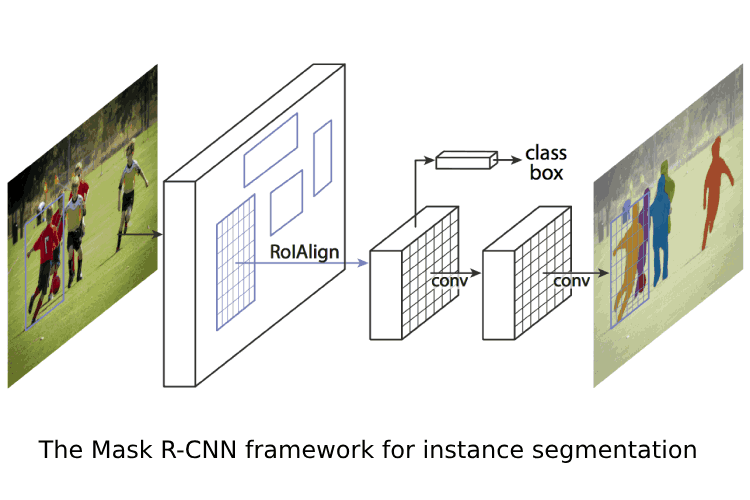
\includegraphics[width=5cm]{images/maskrcnn.png}}
	\caption{The Mask-RCNN architecture}
	\label{maskrcnn}
\end{figure}

The tasks of bladder and prostate segmentation are similar. The images are received as bytes, which are converted to an NRRD (Nearly Raw Raster Data) file. The file data is parsed and each slice is converted into a PNG image file. Figure \ref{flow2} shows the flow of the data from this point on.

\begin{minipage}{0.5\textwidth}
\begin{figure}[H]
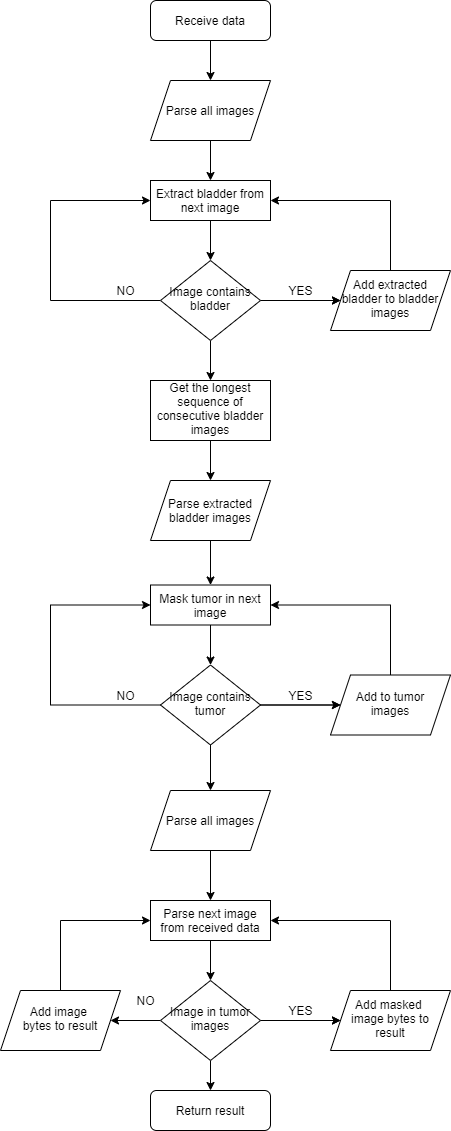
\includegraphics[width=9cm,left]{images/flow_app.png}
\end{figure} \label{flow2}
\end{minipage} \hfill
\begin{minipage}{0.45\textwidth}
\begin{itemize}
\item One by one, the images are passed to the bladder segmentation algorithm. The algorithm saves the segmented images to a new location. Only the images that contain the bladder are saved.
\item The tumor segmentation algorithm analyses each image saved during the previous step. The algorithm returns the masks detected in each image.
\item The output is computed by drawing the predicted masks over the original images. The obtained images are converted into bytes, and the resulted array of byte arrays is returned to the client.  
\end{itemize}
\end{minipage}


\chapter{Application (numerical validation)}
\label{chapter:application}

This chapter presents the two chosen approaches, explains the datasets used and details the obtained results.

\section{Methodology}
\label{section:methodology}

This section presents the methods we propose for bladder, bladder tumor, and prostate segmentation.

We decided to employ Facebook's Detectron2 \cite{wu2019detectron2} since it is considered state-of-the-art in many tasks, including instance segmentation. The chosen model is a Mask-RCNN model pre-trained on the COCO dataset. 

\subsection{Bladder Segmentation}

We trained the Detectron2 model using the data described in Section \ref{section:data}, for 1000 epochs, with a learning rate of 0.00025, and one output class for the desired organ (i.e. bladder, in this case). The algorithm outputs a mask outlining the bladder. Then, these results are saved to PNG images, so that they can be used by the tumor segmentation algorithm. We tested two methods for saving these images, described in the next subsection.

\subsection{Bladder Tumor Segmentation}\label{tumorsegm}

For the task of bladder tumor segmentation, we compared two slightly different methods. For both methods, the received image first passes through the bladder segmentation algorithm. Then, the first method takes as input the image outputted by the bladder segmentation, cropped to display only the segmented bladder, with white pixels to make up for the cropped area. We decided to keep the white area in the picture, rather than crop it completely, to maintain equal resolutions for all images. 

\begin{figure}[htbp]
	\centerline{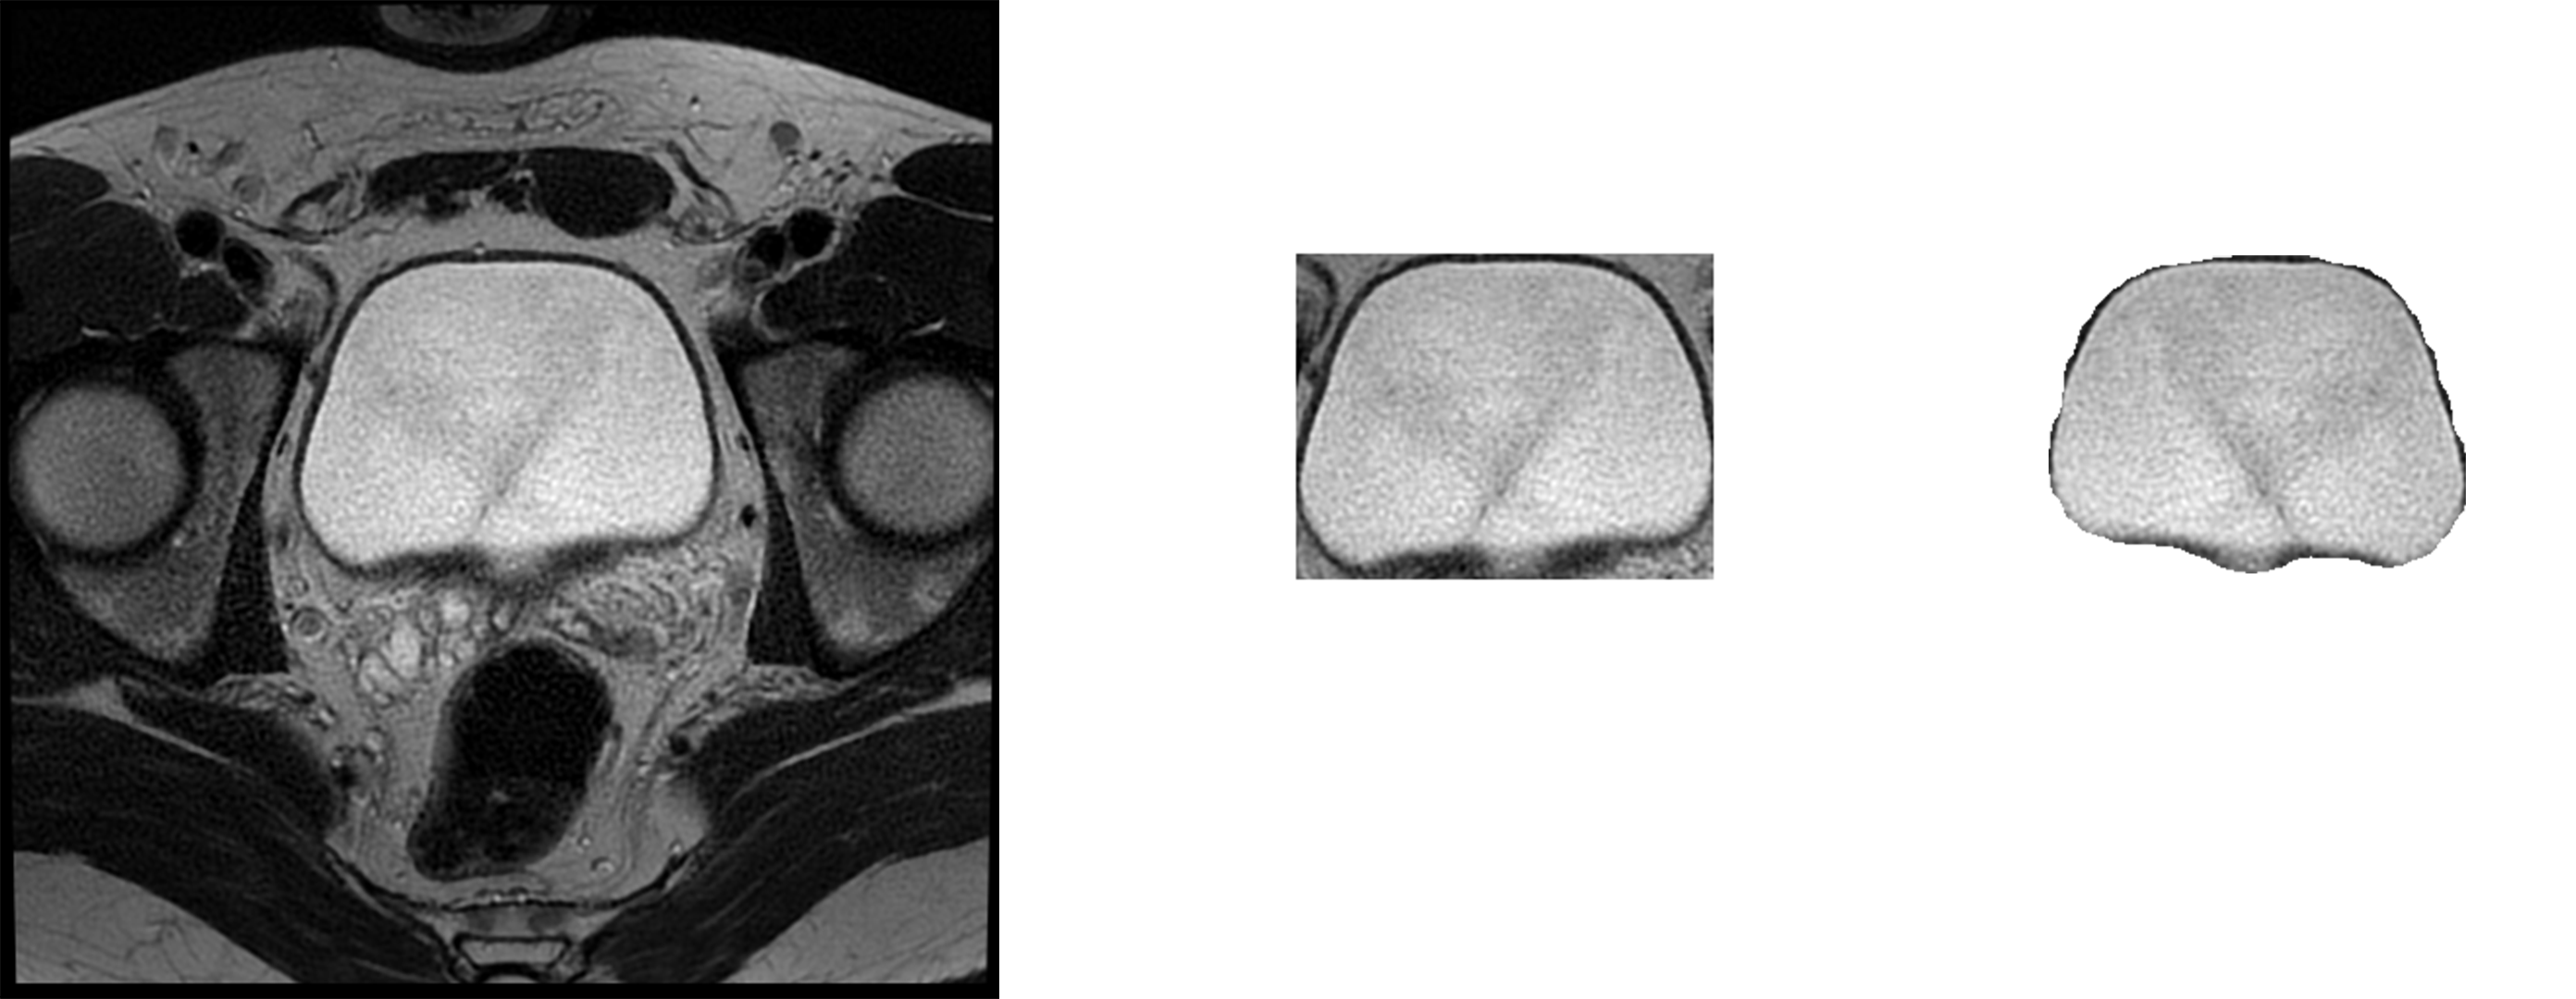
\includegraphics[width=14cm]{images/bladder_6.png}}
	\caption{Left - original image; Center - rectangle cropped around the bladder; Right - the bladder cropped along the outline}
	\label{bladder_6}
\end{figure}

The second method does not use a cropped image, but a masked image. By masked image we mean that the bladder area is segmented precisely, rather than in a rectangle. This modification was used because we remarked that the algorithm sometimes labeled as tumor areas outside the bladder, but within the cropped rectangle. With this modification, we hoped to improve the average IOU of the tumor segmentation model. One bladder slice, along with its cropped and masked segmentations, is displayed in Figure \ref{bladder_6}.

\subsection{Prostate Segmentation}\label{prostatesegm}

For the prostate segmentation task, the algorithm is similar to the bladder segmentation one. The dataset we experimented with, described in Section \ref{prostatedata}, imposed that we test three different methods. In the first method, the model is trained with two output classes, one for the prostate gland and another for the peripheral zone. The second method unifies these areas into one output class for the whole prostate organ. The third method only searches for the central gland, and not the peripheral zone. The results obtained are described in Section \ref{section:results}.

\section{Data}
\label{section:data}

This section describes the datasets used for the proposed algorithm to achieve the results described in Section \ref{section:results}.

\subsection{Bladder Dataset}\label{bladderdata}

For the bladder section of this paper, we used a small dataset from a hospital in Cluj-Napoca, Romania. The dataset consists of 10 patient cases, depicting the bladder captured with an MRI machine, each file having been manually labeled by a different doctor at the hospital. The images came in NRRD (Nearly Raw Raster Data) format. The NRRD files were converted to PNG (Portable Network Graphics) using the nrrd Python library, each file resulting in around 50 PNG slices. All of the images have a resolution of 512x512 pixels.

The organ and the tumors were labeled by creating a polygon around the bladder outline, as well as other polygons around the tumors. This format was difficult to work with so, for ease of use, we labeled the segmentations again using the labelme Python library. These new segmentations were converted into COCO format using a Python script. We used 8 patient cases for training and 2 patient cases for testing. This resulted in 386 images for training and 81 images for testing. Two slice segmentations are displayed in Figure \ref{bladder_1}.

\begin{figure}[htbp]
	\centerline{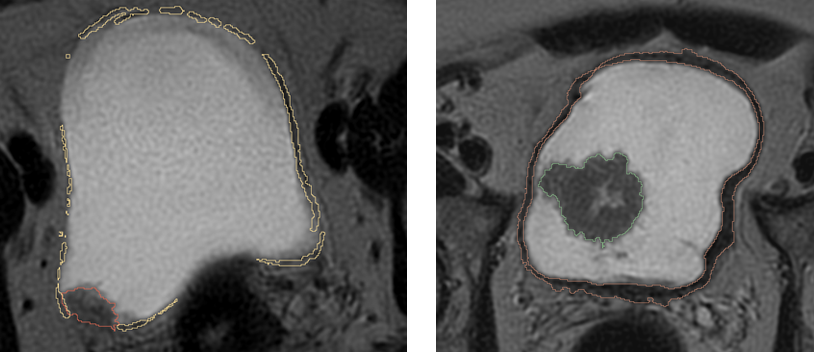
\includegraphics[width=14cm]{images/bladder_1.png}}
	\caption{Segmentations of two bladder slices - images obtained from a hospital in Cluj-Napoca, Romania - On the left, the yellow contour outlines the bladder and the red contour outlines the tumor. On the right, the red contour outlines the bladder and the green contour outlines the tumor.}
	\label{bladder_1}
\end{figure}

\subsection{Prostate Dataset}\label{prostatedata}

For the prostate section of this paper, we used part of the NCI-ISBI 2013 Challenge dataset, called PROSTATE-DIAGNOSIS, obtained from the Cancer Imaging Archive. This dataset is made up of 30 patient cases. 

\begin{figure}[htbp]
	\centerline{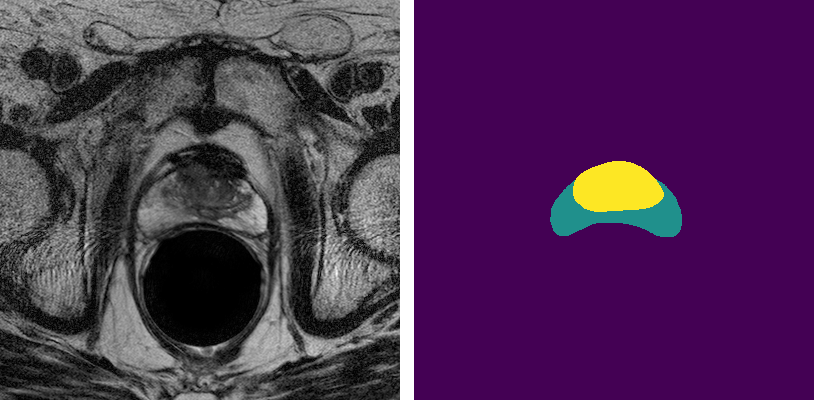
\includegraphics[width=10cm]{images/prostate_1.png}}
	\caption{Side-by-side of one prostate slice and its segmentation - image obtained from the Prostate-Diagnosis dataset - Yellow represents the central gland (CG) and blue represents the peripheral zone (PZ)}
	\label{prostate_1}
\end{figure}

Each file comes in NRRD format, with 30 to 40 slices. The slices were converted to PNG, obtaining 966 images. These images were split into 802 for training and 164 for testing. The images have a resolution of 400x400 pixels. The segmentations also came in NRRD format, but we handled this dataset differently. We converted the segmentations into PNG images, then used a Python script to convert the mask represented in the image into COCO format. One slice, as well as its segmentation, can be seen in Figure \ref{prostate_1}.

\section{Results}
\label{section:results}

This section details the obtained results for the task of bladder segmentation, bladder tumor segmentation, and prostate segmentation. All of these results were obtained by computing the Intersection Over Union (IOU) value and the Dice Similarity Coefficient (DSC). The IOU was computed by combining the detected and the expected polygons into binary masks, computing the sum of the masks, and dividing the number of elements with the value 2 to the number of elements with a value greater than 0. The Dice Similarity Coefficient (DSC) was similarly computed by multiplying the intersection by 2 and dividing the result by the sum of the number of pixels in both of the masks.

\subsection{Bladder Segmentation}

As mentioned previously, we tested the bladder segmentation algorithm on 2 out of 10 patient cases, resulting in 81 images. We obtained an IOU value of 93.41\% and a DSC of 95.69\%. For comparison, the IOU value was also computed on the training set, obtaining a value of 94.35\%. During development, we noticed and addressed a number of issues:

\begin{figure}[!tbp]
  \centering
  \begin{minipage}[b]{0.4\textwidth}
    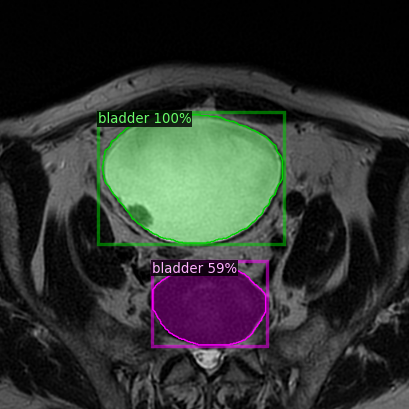
\includegraphics[width=\textwidth]{images/bladder_2.png}
    \caption{Case where the algorithm detects two bladders} \label{bladder_2}
  \end{minipage}
  \hfill
  \begin{minipage}[b]{0.4\textwidth}
    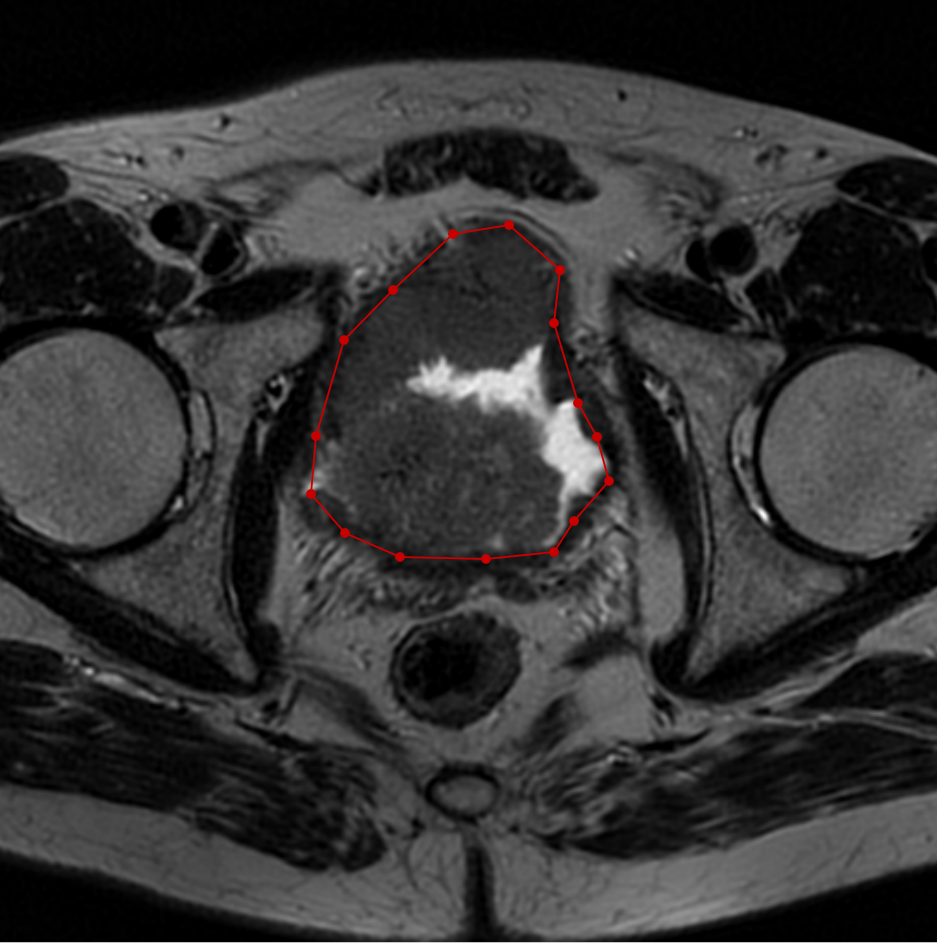
\includegraphics[width=\textwidth]{images/bladder_3.png}
    \caption{Case where the tumor covers most of the bladder} \label{bladder_3}
  \end{minipage}
\end{figure}

\begin{itemize}
    \item The algorithm sometimes detects two areas as being the bladder. We solved this issue by returning only the area with the highest confidence level. Such a case is displayed in Figure \ref{bladder_2}.
    \item The algorithm started to detect the bladder even in the first and last slices, when the organ was so small that it remained unlabeled. We solved this issue by manually labeling the first and last slices.
    \item The algorithm sometimes detects the bladder in slices where there should not be one, usually far away from where the bladder slices actually begin and end. We solved this issue by returning the longest sequence of slices where the bladder is detected. This way, the detected slices that do not connect to the actual bladder will be ignored.
    \item The algorithm has issues when the tumor is big enough to cover most of the bladder. This is to be expected, since there is little to no difference between the aspect of the bladder wall tissue and the tumor tissue. Such a case is displayed in Figure \ref{bladder_3}.
\end{itemize}

\begin{figure}[htbp]
	\centerline{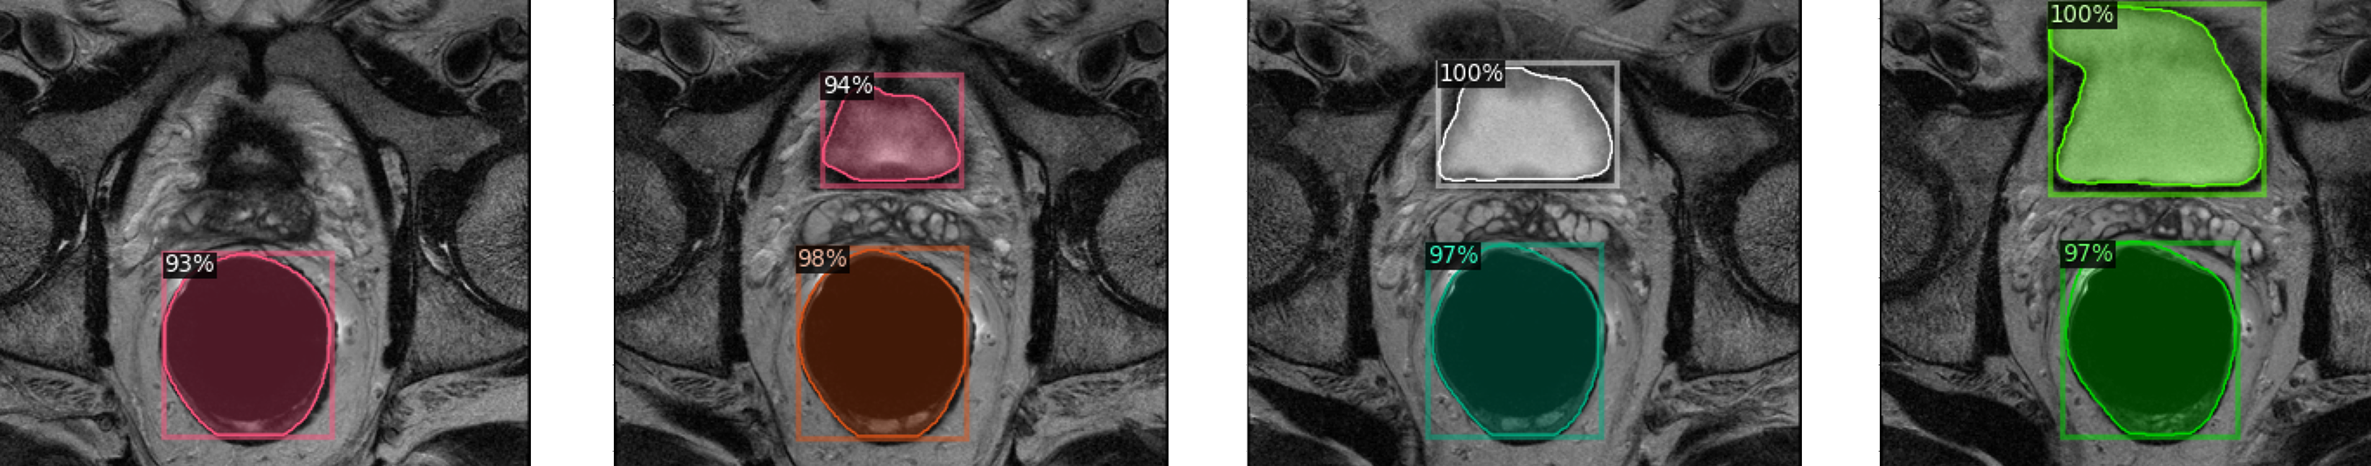
\includegraphics[width=17cm]{images/bladder_4.png}}
	\caption{Performance of the bladder segmentation algorithm on the prostate dataset - In the first image, the bladder is too small to be detected, but there is a very confident false positive. In the second image, it detects both the bladder and the false positive, but only returns the false positive, since the confidence is higher. In the third and fourth images, the bladder confidence is greater than the false positive, so the bladder mask is accurately returned.}
	\label{bladder_4}
\end{figure}

We also ran the bladder segmentation algorithm on the prostate dataset, for comparison. The algorithm performs well on slices containing the bladder, but has many false positives on other slices. Such a comparison is displayed in Figure \ref{bladder_4}.

\subsection{Bladder Tumor Segmentation - Method 1}\label{method1}

For the tumor segmentation task, with the first method described in Section \ref{tumorsegm} we obtained an IOU of 77.11\%. We noticed that when the bladder is very small, on slices at the beginning and end, it is inaccurately labeled as a tumor. One such slice is shown in Figure \ref{bladder_5}, side by side with the next slice, which is accurately left unlabeled. When removing these problematic slices from the computation, the obtained IOU value is 86.75\%.

\begin{figure}[htbp]
	\centerline{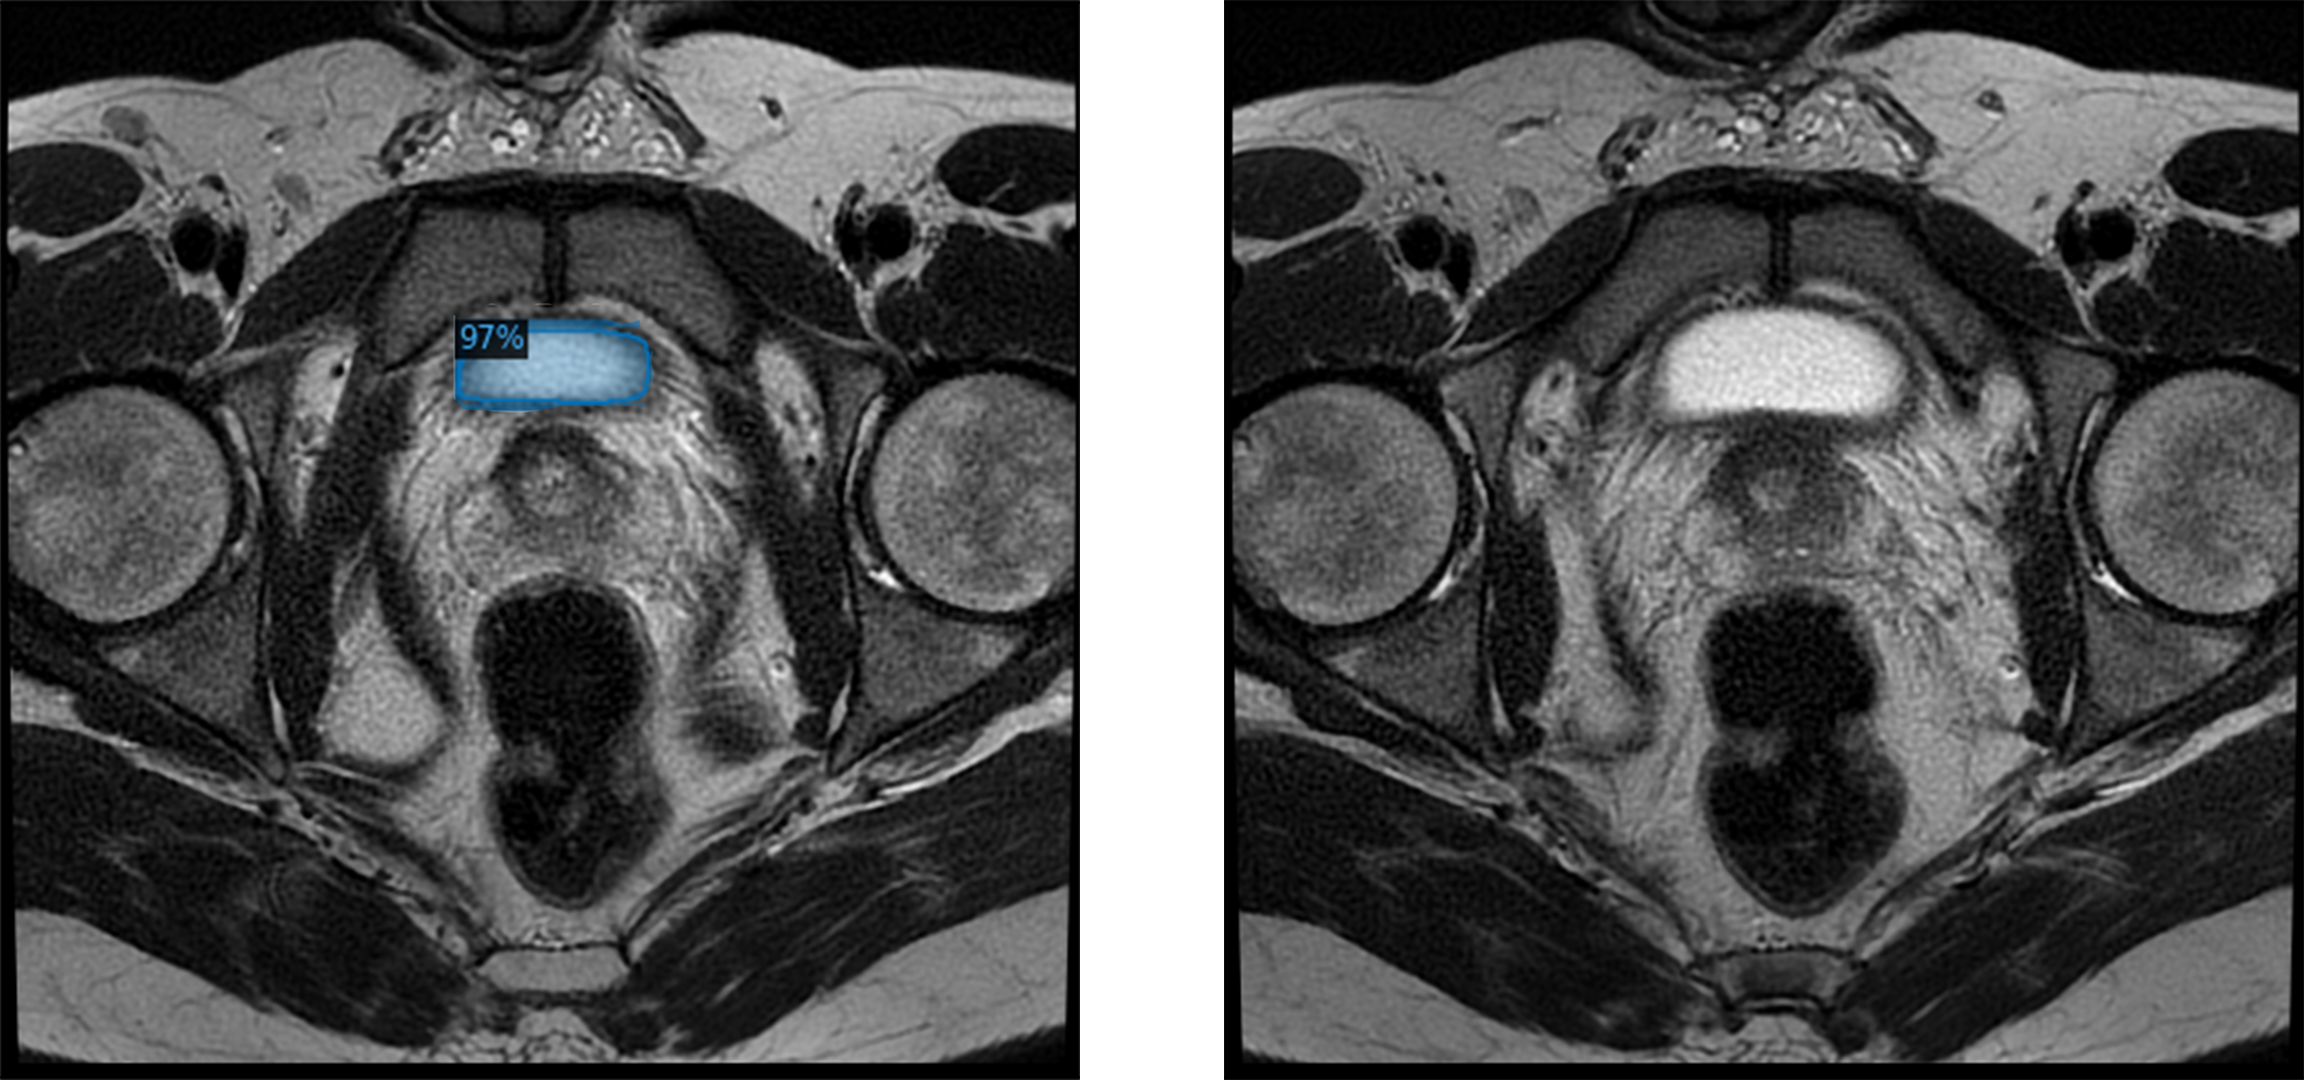
\includegraphics[width=17cm]{images/bladder_5.png}}
	\caption{Problematic slice for the task of bladder tumor segmentation - On the left, the first slice of the bladder is inaccurately labeled as a tumor. On the right, the second slice of the bladder is accurately left unlabeled.}
	\label{bladder_5}
\end{figure}

For comparison, we computed the IOU value on the training dataset as well. When including the problematic slides, we obtained a value of 80.53\%, and a DSC of 82.14\%. When they were removed, the IOU value grew to 84.31\%.

\subsection{Bladder Tumor Segmentation - Method 2}

For the tumor segmentation task, with the second method described in Section \ref{tumorsegm} we obtained an IOU of 80.68\%. After removing the problematic slices described in Subsection \ref{method1}, the IOU value grew to 89.1\%. On the training set, the IOU value is 82.33\% with the problematic slices, and 89.9\% without. The results show that the second method clearly outperforms the first one because the false positives around the bladder, but within the cropped rectangle, are omitted.

\subsection{Prostate Segmentation}

The results for the task of prostate segmentation are rather poor. The quality of the dataset is lacking and there is a need for image preprocessing and result postprocessing to obtain a better performance. We chose not to compute the evaluation metrics for the prostate segmentation task because it was clearly visible that the numerical performance would be disappointing. Two segmented prostate slices can be seen in Figure \ref{prostate2}.

\begin{figure}[htbp]
	\centerline{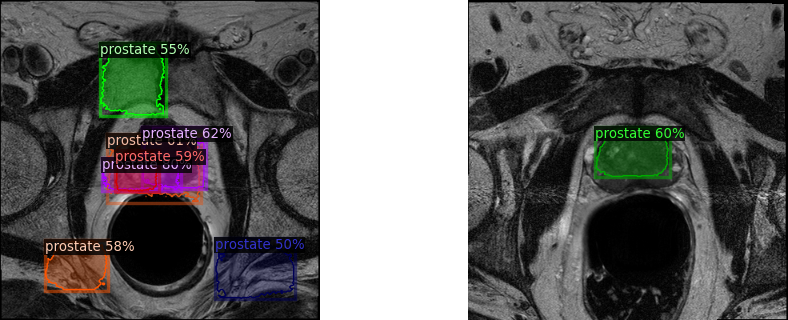
\includegraphics[width=17cm]{images/prostate2.png}}
	\caption{Left - poorly segmented slice of a prostate MRI scan; Right - a slightly better segmentation which proves that a better dataset could increase the performance}
	\label{prostate2}
\end{figure}

The best results, however poor, were obtained for the third method described in Subsection \ref{prostatesegm}, which only segments the central gland. This implies that in future improvements, we might need two different models, one to segment the gland, and another to segment the peripheral zone.

\section{In practice}
\label{section:practice}

To prove the utility of our approach, we integrated the intelligent algorithms within an Application Programming Interface (API). This API was then utilized in the development of an application meant to assist medical students or doctors in correctly diagnosing their patients and tracking the progress of their illness. The flow of the application can be seen in the flowchart diagram in Figure \ref{flowchart}.

\begin{figure}[htbp]
	\centerline{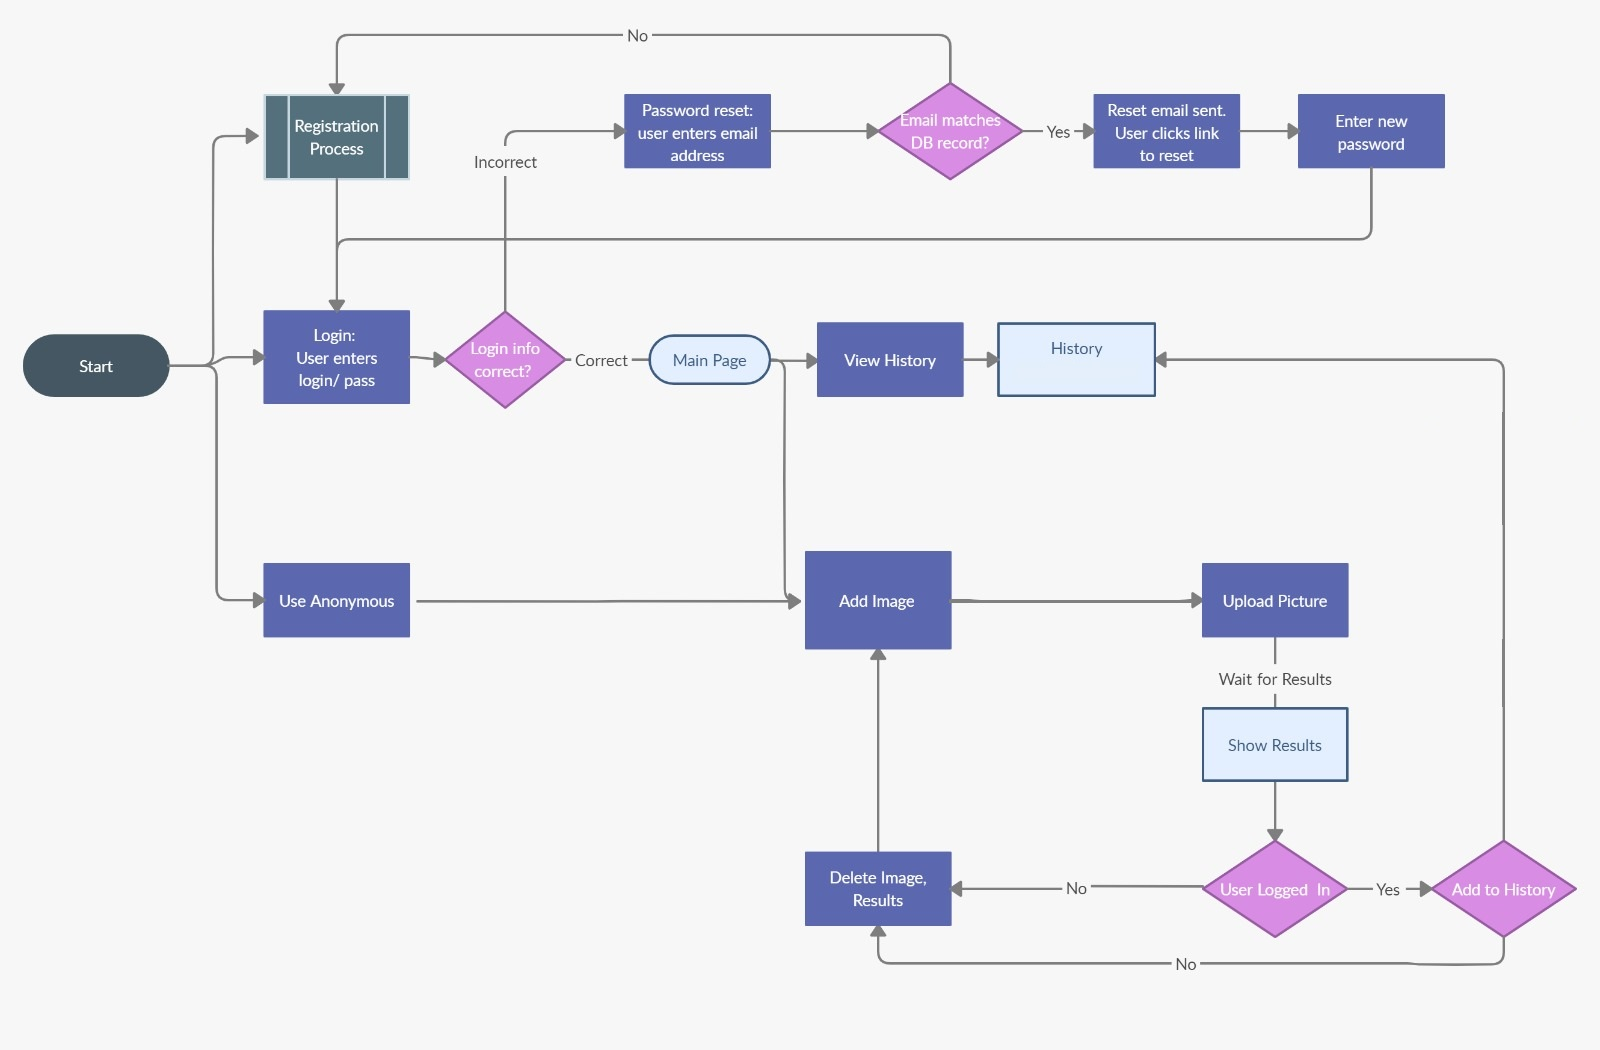
\includegraphics[width=17cm]{images/flow.jpg}}
	\caption{The Flowchart Diagram of our proposed application}
	\label{flowchart}
\end{figure}

The intelligent algorithms and the API were implemented using Python (Flask). The server handles tasks such as logging in, registering, saving and displaying a user's history, uploading and analysing images and retrieving the results. The data is stored in an SQL database. The structure of the database is displayed in Figure \ref{database}.

\begin{figure}[htbp]
	\centerline{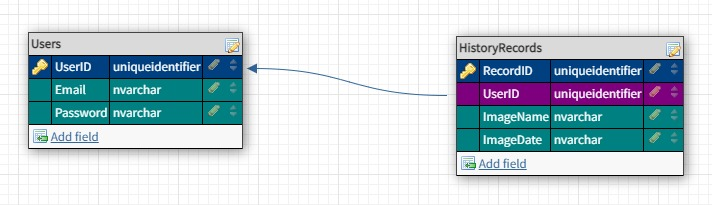
\includegraphics[width=17cm]{images/database.jpeg}} 
	\caption{The Class Diagram of our proposed application}
	\label{database}
\end{figure}

\subsection{The website interface}

The frontend component of our application was implemented using Angular. The design is a minimalist one, that incorporates smooth animations that provide to the user a great experience. The colors and the fonts are outstanding in order to help the user understand the flow better. The application consists of five pages: the main page which the user sees first when landing on the website, the quick analysis page, the login and register page, the results page and the history page. In figure \ref{frontend_dashboard} it can be seen the first page that the users can see and find out some details about the purpose of the application. 

\begin{figure}[h!]
	\centerline{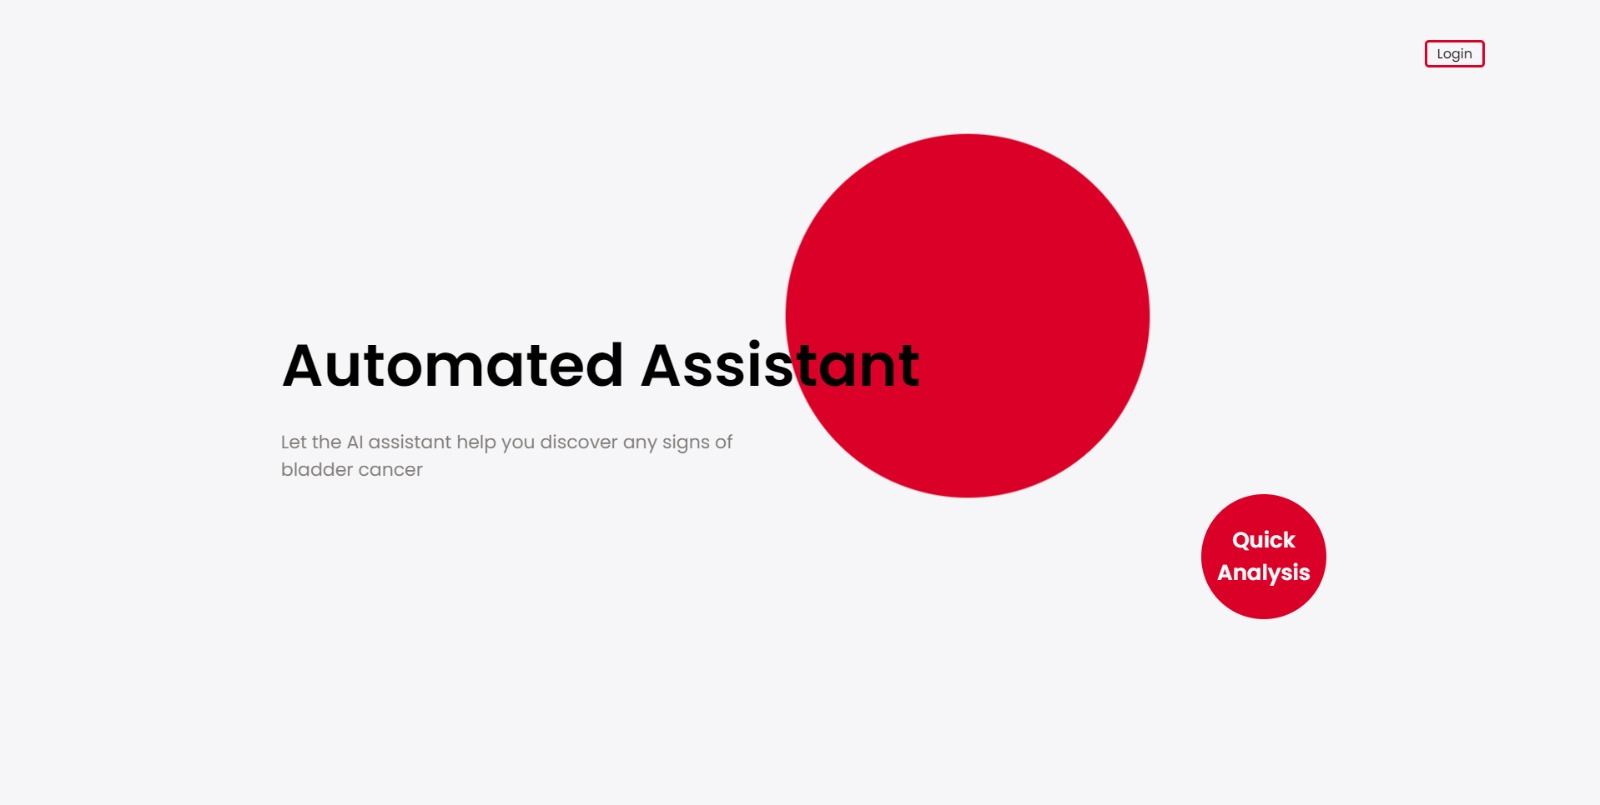
\includegraphics[width=17cm]{images/frontend_dashboard.jpeg}} 
	\caption{The main page of our proposed application}
	\label{frontend_dashboard}
\end{figure}

Here there is the option of going to the analysis page for a quick analyse. It should be noted that if the user is not logged in, the results of the analyse will not be saved for the user to access it later. Together with the "Quick Analysis" button, one can also find the "Login" button that can be accessed in order to redirect to the login page, as seen in \ref{frontend_login}.

\begin{figure}[h!]
	\centerline{
\includegraphics[width=17cm]{images/frontend_login.jpeg}} 
	\caption{Login page}
	\label{frontend_login}
\end{figure}

 At this stage, the user can login, or can register in case he or she doesn't have an account. By clicking on the pencil icon, the register form will appear and the user can fill in the email and the password fields as shown in \ref{frontend_register}. 

\begin{figure}[h!]
	\centerline{
\includegraphics[width=17cm]{images/frontend_register.jpeg}}
	\caption{Register page}
	\label{frontend_register}
\end{figure}

After clicking the "NEXT" button, a toast element will pop up showing if the action was successful or not. After the user registers, the login form will show again and it will give the user the possibility to login. After a successful login, the analyse page will be displayed, as presented in \ref{frontend_analyse}.

\begin{figure}[h!]
	\centerline{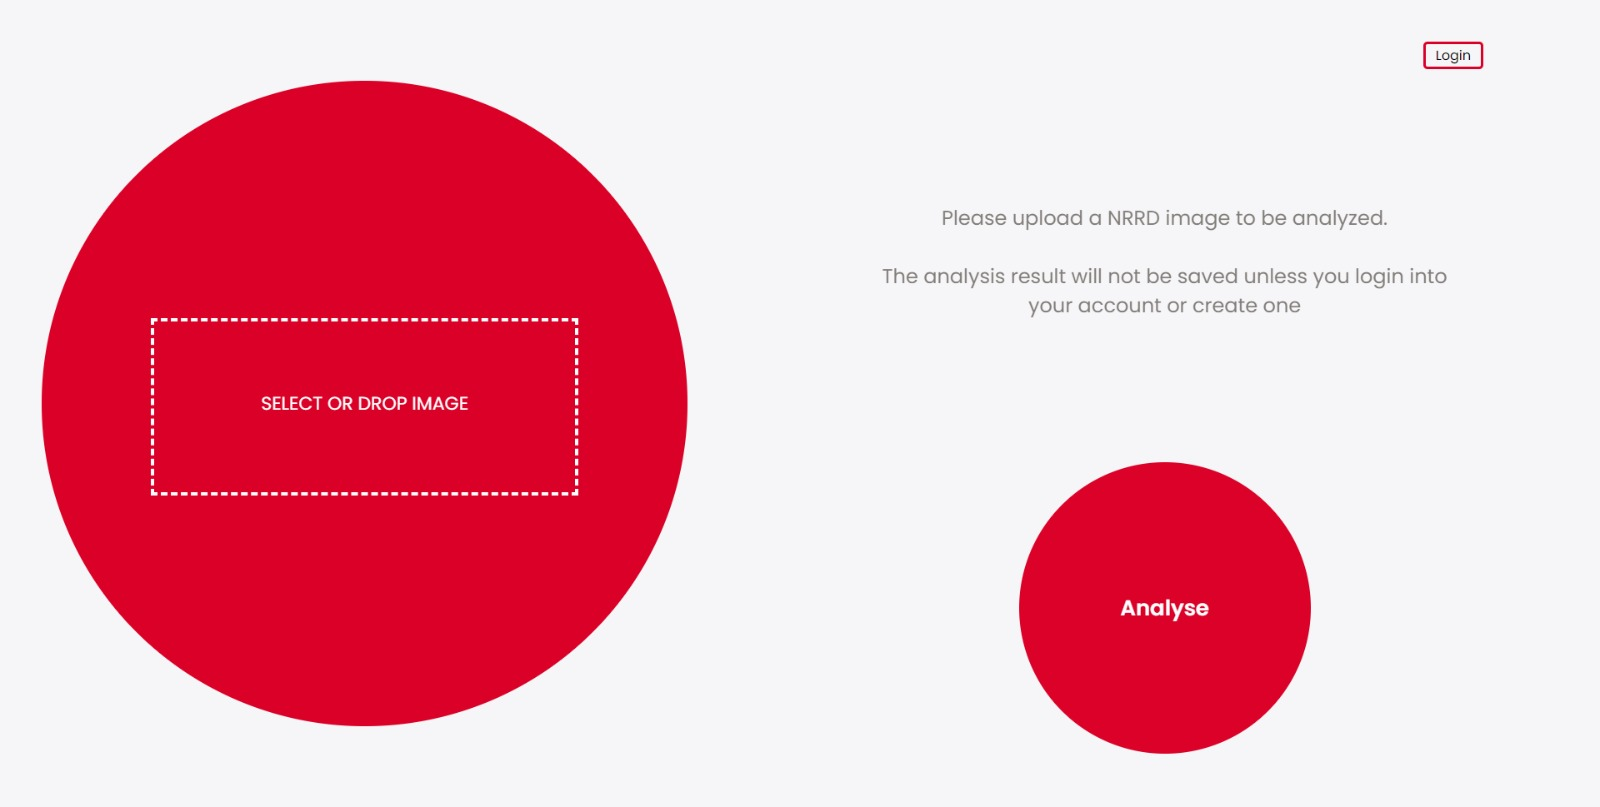
\includegraphics[width=17cm]{images/frontend_analyse.jpeg}}
	\caption{Analyse page}
	\label{frontend_analyse}
\end{figure}

Once reached at the this stage, the user can now upload an image of its choice. Currently the application only accepts .jpg, jpeg, .png and .nrrd type files. After uploading the image, the user has also the option to remove it, in case the image is not the correct one. By clicking the "Analyse" button, the image will be sent to be processed. A custom cross loader will show up until the results are received. Once the results arrive, they will be displayed in a different page, as shown in \ref{frontend_result}.

\begin{figure}[h!]
	\centerline{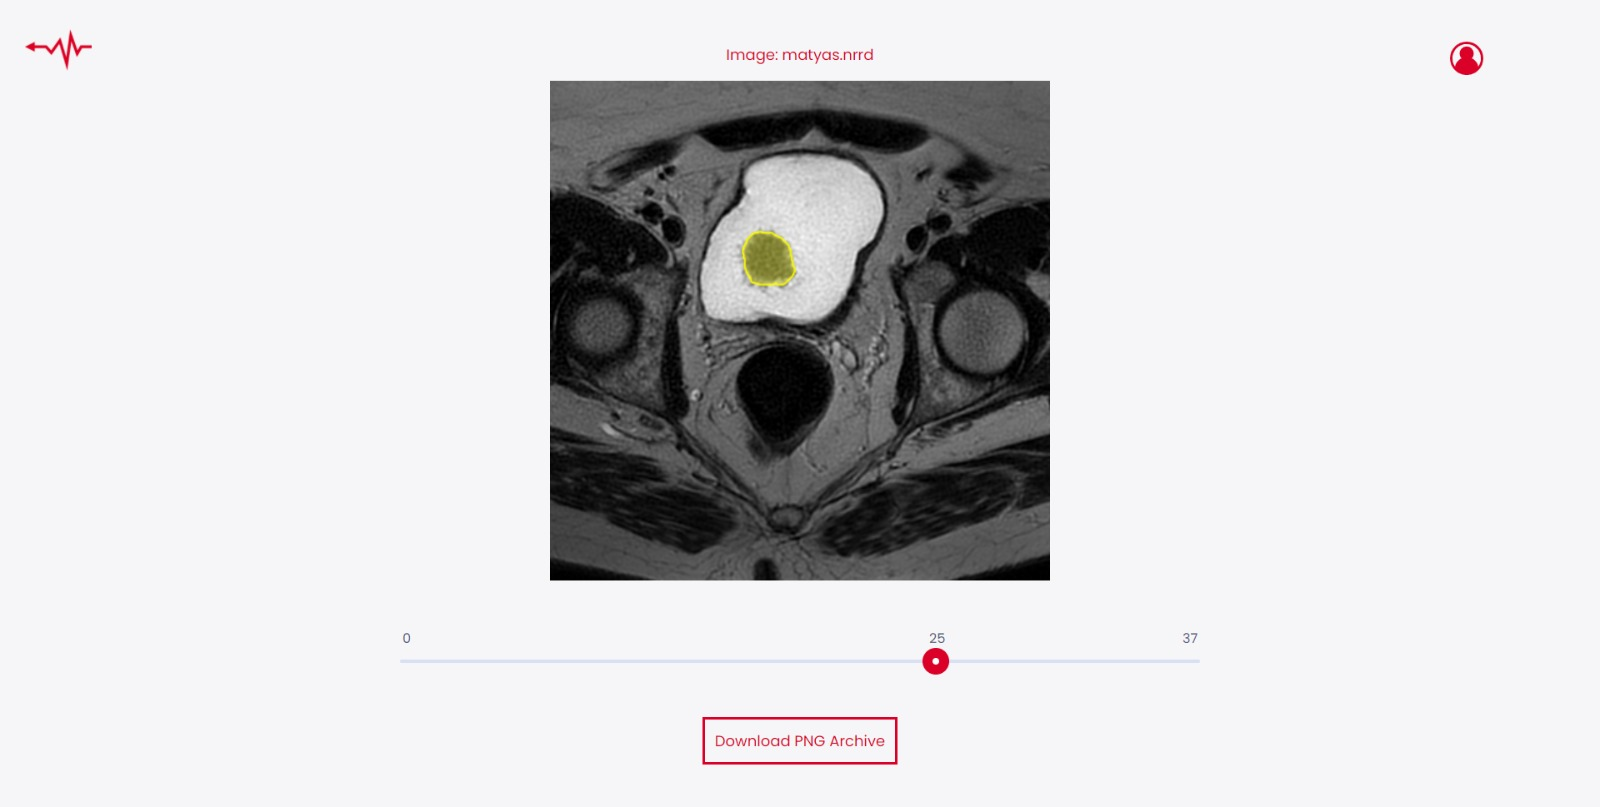
\includegraphics[width=17cm]{images/frontend_result.jpeg}}
	\caption{Results page}
	\label{frontend_result}
\end{figure}

The results page will display a slider of images that represent the result of the analysis. At this point, the user has the possibility to download an archive of the resulted PNG images by clicking the "Download PNG Archive" button.

\begin{figure}[h!]
	\centerline{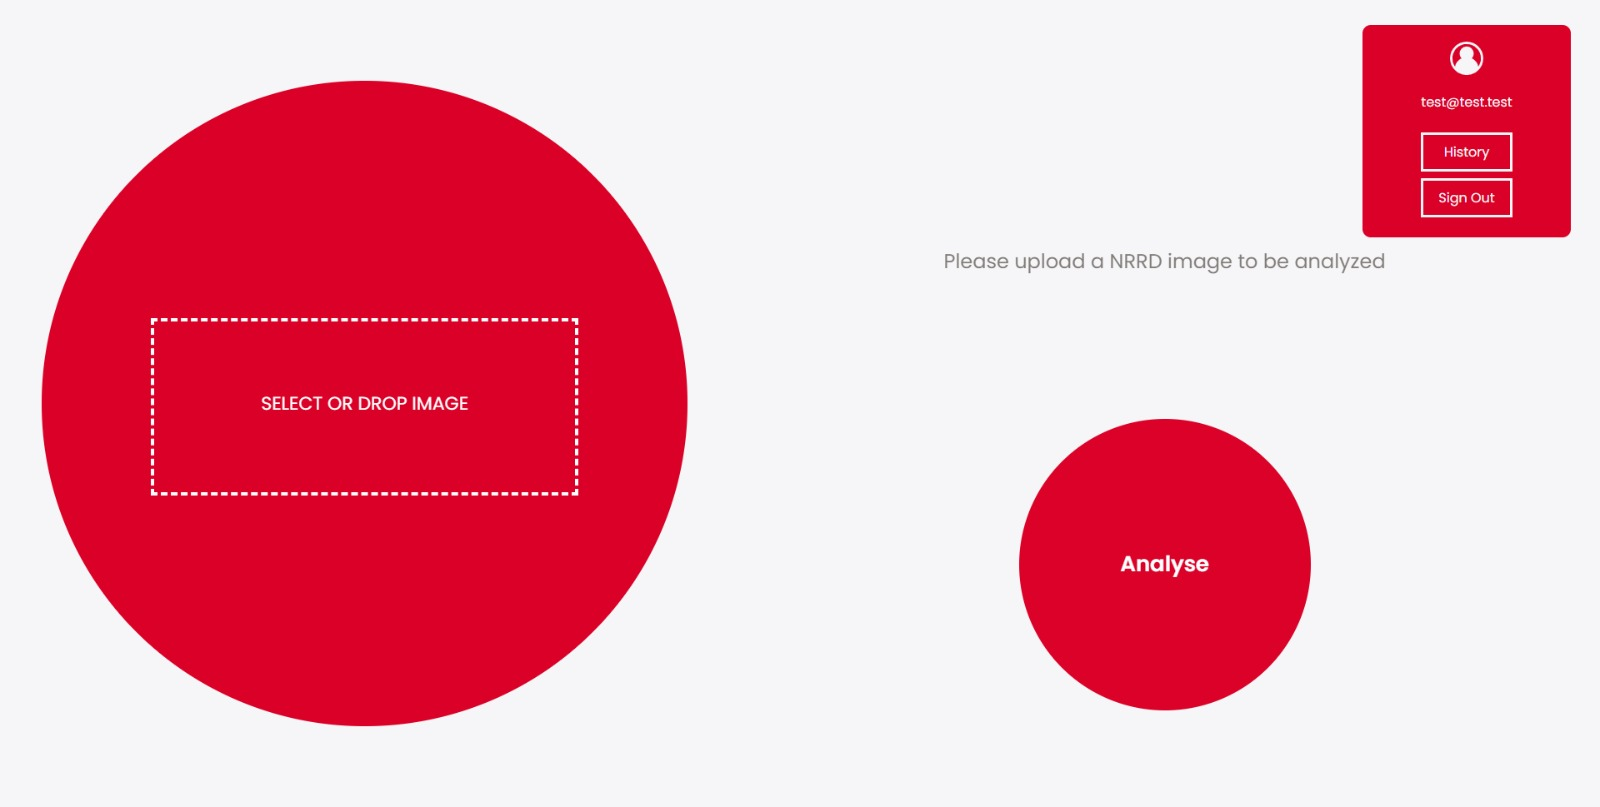
\includegraphics[width=17cm]{images/frontend_userDetails.jpeg}}
	\caption{User details}
	\label{frontend_userDetails}
\end{figure}

In \ref{frontend_userDetails} it can be seen that if the user icon is hovered, the details of the user will be displayed, together with a "Sign Out" button that will logout the user and a "History" button. By clicking the last button mentioned, the history page will appear, as it can be observed in \ref{frontend_history}.

\begin{figure}[h!]
	\centerline{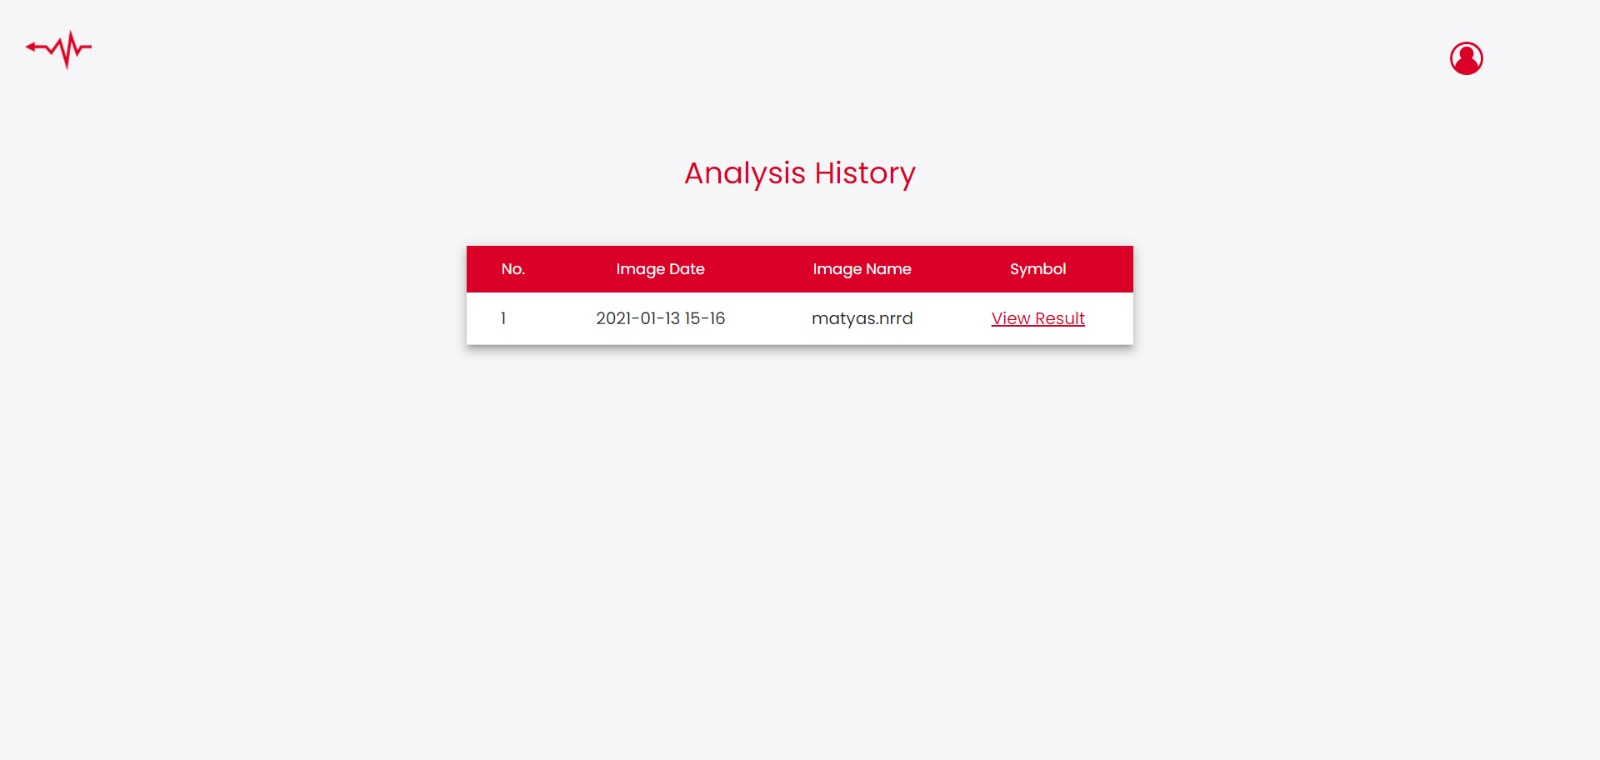
\includegraphics[width=17cm]{images/frontend_history.jpeg}}
	\caption{History page}
	\label{frontend_history}
\end{figure}

This page displays a table containing the information for every image analysed by the logged in user: the date when the images has been processed, the image name and a link to the results of the image. When the link is being clicked, the results will be displayed in the Results page as presented in \ref{frontend_result}.


\vspace{4cm}

\chapter{Conclusion and future work}
\label{chapter:concl}

Bladder cancer is the forth most common cancer type presented in men. It has a 5-year survival rate of 96\% for the 1\textsuperscript{st} stage, 70\% for the 2\textsuperscript{nd} stage, 36\% for the 3\textsuperscript{rd} stage, and only 5\% for the 4\textsuperscript{th} stage. Taking into consideration these statistics, it is absolutely necessary for the tumor to be discovered in the earliest stage. Nowadays, the advanced technology is capable of automating this process and drastically decreasing the evaluation time of the radiographs. 

The proposed application presented in this paper has the purpose of solving this problem, by efficiently providing an almost accurate segmentation of the bladder in order for the doctors to interpret it faster. The application uses a client-server approach that has a web application constructed in Angular as its client and a server constructed in Python by using the Flask technology. 

In addition to the presented implementation of the solution, we would like to include several future improvements such as: the possibility to automatically segment the prostate organ and tumors, the possibility to import a larger variety of image type files, an interactive 3D representation of the results and an interpretation map for the resulted images. 

\bibliographystyle{plain}
\bibliography{bib.bib}

\end{document}
